\chapter{Exponential distribution and its extensions}
%%%%%%%%%%%%%%%%%%%%%%%%%%%%%%%%%%%%%%%%%%%%%%%
\section{Exponential distribution}
\subsection{Characterization}
\begin{wrapfigure}{r}{0.5\textwidth}
  \vspace{-20pt}
  \begin{center}
    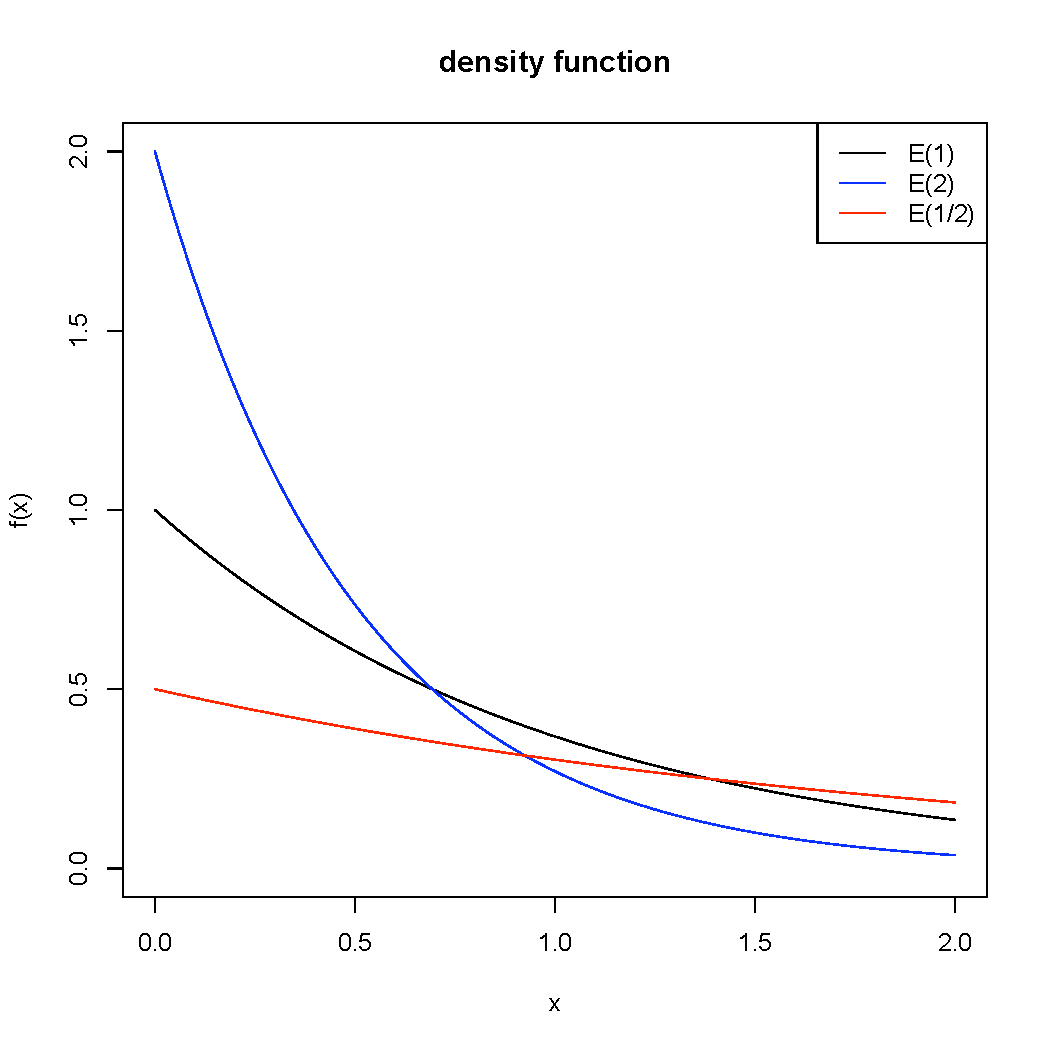
\includegraphics[width=0.48\textwidth]{img/expzoom}
  \end{center}
  \vspace{-20pt}  
  \caption{Density function for exponential distributions}
%  \vspace{-20pt}  
\end{wrapfigure}

The exponential is a widely used and widely known distribution. It is characterized
by the following density
$$
f(x) = \lambda e^{-\lambda x},
$$
for $x>0$ and $\lambda >0$. Its distribution function is
$$
F(x) =  1-e^{-\lambda x}.
$$

Since it is a light-tailed distribution, the moment generating function of an exponential distribution 
$\mathcal E(\lambda)$ exists which is
$$
M(t)=\frac{\lambda}{\lambda -t},
$$
while its characteristic function is 
$$
\phi(t) = \frac{\lambda}{\lambda-it}.
$$

\subsection{Properties}
The expectation and the variance of an exponential distribution $\mathcal E(\lambda)$
are $\frac{1}{\lambda}$ and $\frac{1}{\lambda^2}$. Furthermore the $n$-th moment is given
by 
$$
E(X^n) = \frac{\Gamma(n+1)}{\lambda^n}.
$$

The exponential distribution is the only one continuous distribution to verify the lack of memory property. That is to say if $X$ is exponentially distributed, we have
$$
\frac{P(X>t+s)}{P(X>s)} = P(X>t),
$$
where $t,s>0$.

If we sum $n$ i.i.d. exponentially distributed random variables, we get a gamma distribution $\mathcal G(n,\lambda)$.

\subsection{Estimation}
The maximum likelihood estimator and the moment based estimator are the same
$$
\hat \lambda = \frac{n}{\sum_{i=1}^n X_i} = \frac{1}{\overline X_n},
$$
for a sample $(X_i)_{1\leq i\leq n}$. But the unbiased estimator with mininum variance
is 
$$
\tilde \lambda  = \frac{n-1}{\sum_{i=1}^n X_i}.
$$
Exact confidence interval for parameter $\lambda$ is given by 
$$
I_\alpha(\lambda) = \left[ \frac{z_{2n,1-\frac{\alpha}{2}} }{2\sum_{i=1}^n X_i} , \frac{z_{2n,\frac{\alpha}{2}} }{2\sum_{i=1}^n X_i} \right],
$$
where $z_{n,\alpha}$ denotes the $\alpha$ quantile of the chi-squared distribution.

\subsection{Random generation}
Despite the quantile function is $F^{-1}(u)=-\frac{1}{\lambda}\log(1-u)$, generally the exponential distribution $\mathcal E(\lambda)$ is generated by applying $-\frac{1}{\lambda}\log(U)$ on 
a uniform variate $U$.

\subsection{Applications}
From wikipedia, the exponential distribution occurs naturally when describing the lengths of the inter-arrival times in a homogeneous Poisson process.

The exponential distribution may be viewed as a continuous counterpart of the geometric distribution, which describes the number of Bernoulli trials necessary for a ''discrete'' process to change state. In contrast, the exponential distribution describes the time for a continuous process to change state.

In real-world scenarios, the assumption of a constant rate (or probability per unit time) is rarely satisfied. For example, the rate of incoming phone calls differs according to the time of day. But if we focus on a time interval during which the rate is roughly constant, such as from 2 to 4 p.m. during work days, the exponential distribution can be used as a good approximate model for the time until the next phone call arrives. Similar caveats apply to the following examples which yield approximately exponentially distributed variables:
\begin{itemize}
\item the time until a radioactive particle decays, or the time between beeps of a geiger counter;
\item the time it takes before your next telephone call
\item the time until default (on payment to company debt holders) in reduced form credit risk modeling
\end{itemize}

Exponential variables can also be used to model situations where certain events occur with a constant probability per unit ''distance'':
\begin{itemize}
\item the distance between mutations on a DNA strand;
\item the distance between roadkill on a given road;
\end{itemize}

In queuing theory, the service times of agents in a system (e.g. how long it takes for a bank teller etc. to serve a customer) are often modeled as exponentially distributed variables.  (The inter-arrival of customers for instance in a system is typically modeled by the Poisson distribution in most management science textbooks.)  The length of a process that can be thought of as a sequence of several independent tasks is better modeled by a variable following the Erlang distribution (which is the distribution of the sum of several independent exponentially distributed variables).

Reliability theory and reliability engineering also make extensive use of the exponential distribution. Because of the ``memoryless'' property of this distribution, it is well-suited to model the constant hazard rate portion of the bathtub curve used in reliability theory. It is also very convenient because it is so easy to add failure rates in a reliability model.
The exponential distribution is however not appropriate to model the overall lifetime of organisms or technical devices, because the ``failure rates'' here are not constant: more failures occur for very young and for very old systems.

In physics, if you observe a gas at a fixed temperature and pressure in a uniform gravitational field, the heights of the various molecules also follow an approximate exponential distribution. This is a consequence of the entropy property mentioned below.


%%%%%%%%%%%%%%%%%%%%%%%%%%%%%%%%%%%%%%%%%%%%%%%
\newpage
\section{Shifted exponential}
\subsection{Characterization}
\begin{wrapfigure}{r}{0.5\textwidth}
  \vspace{-20pt}
  \begin{center}
    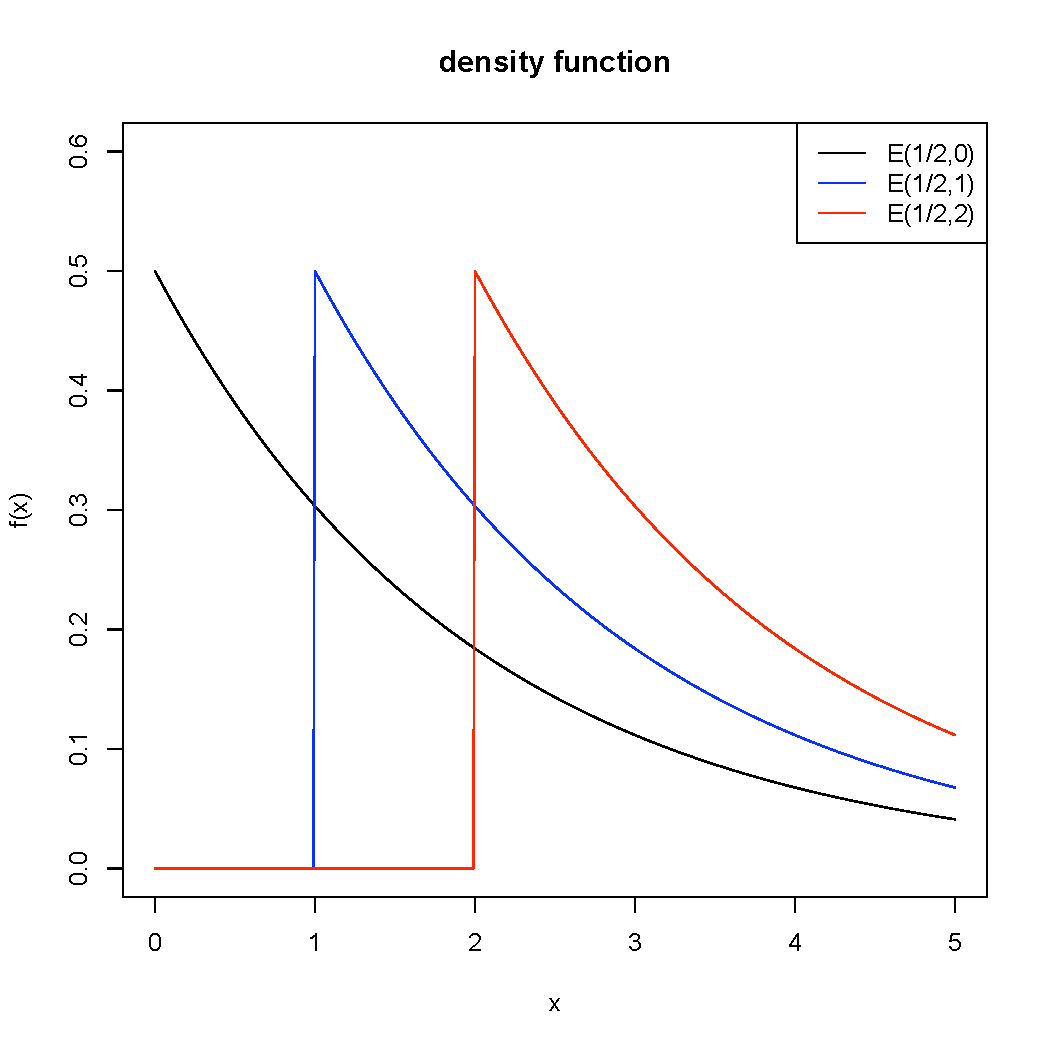
\includegraphics[width=0.48\textwidth]{img/shiftexpzoom}
  \end{center}
  \vspace{-20pt}  
  \caption{Density function for shifted exponential distributions}
\end{wrapfigure}
The distribution of the shifted exponential distribution is simply the distribution of $X-\tau$ when $X$ is exponentially distributed. Therefore the density is given by
$$
f(x) = \lambda e^{-\lambda(x-\tau)}
$$
for $x>\tau$.
The distribution function is given by
$$
F(x) = 1-e^{-\lambda(x-\tau)}
$$
for $x>\tau$.

As for the exponential distribution, there exists a moment generating function
$$
M(t) = e^{-t\tau} \frac{\lambda}{\lambda-t}
$$
and also a characteristic function
$$
\phi(t) = e^{-it\tau} \frac{\lambda}{\lambda-it}.
$$

\subsection{Properties}
The expectation and the variance of an exponential distribution $\mathcal E(\lambda,\tau)$
are $\tau+\frac{1}{\lambda}$ and $\frac{1}{\lambda^2}$. 

Furthermore the $n$-th moment (for $n$ integer) is computable with the binomial formula by 
$$
E(X^n) = \sum_{i=0}^n \frac{n!}{(n-i)!} \frac{(-\tau)^n}{(-\lambda\tau)^i}.
$$

\subsection{Estimation}
Maximum likelihood estimator for $\tau$ and $\lambda$ are given by
$$
\hat \tau = X_{1:n}
\txtm{and}
\hat \lambda = \frac{n}{\sum_{i=1}^n(X_i-\hat \tau)}
$$
where $X_{i:n}$ denotes the $i$th order statistic. Since the minimum $X_{1:n}$ follows a shifted exponential distribution $\mcal E(n\lambda,\tau)$, we have $\hat \tau$ is biased but asympotically unbiased.

NEED REFERENCE for unbiased estimators

\subsection{Random generation}
The random generation is simple: just add $\tau$ to the algorithm of exponential distribution.

\subsection{Applications}
NEED REFERENCE

%%%%%%%%%%%%%%%%%%%%%%%%%%%%%%%%%%%%%%%%%%%%%%%
\section{Inverse exponential}
\subsection{Characterization}
\begin{wrapfigure}{r}{0.5\textwidth}
  \vspace{-20pt}
  \begin{center}
    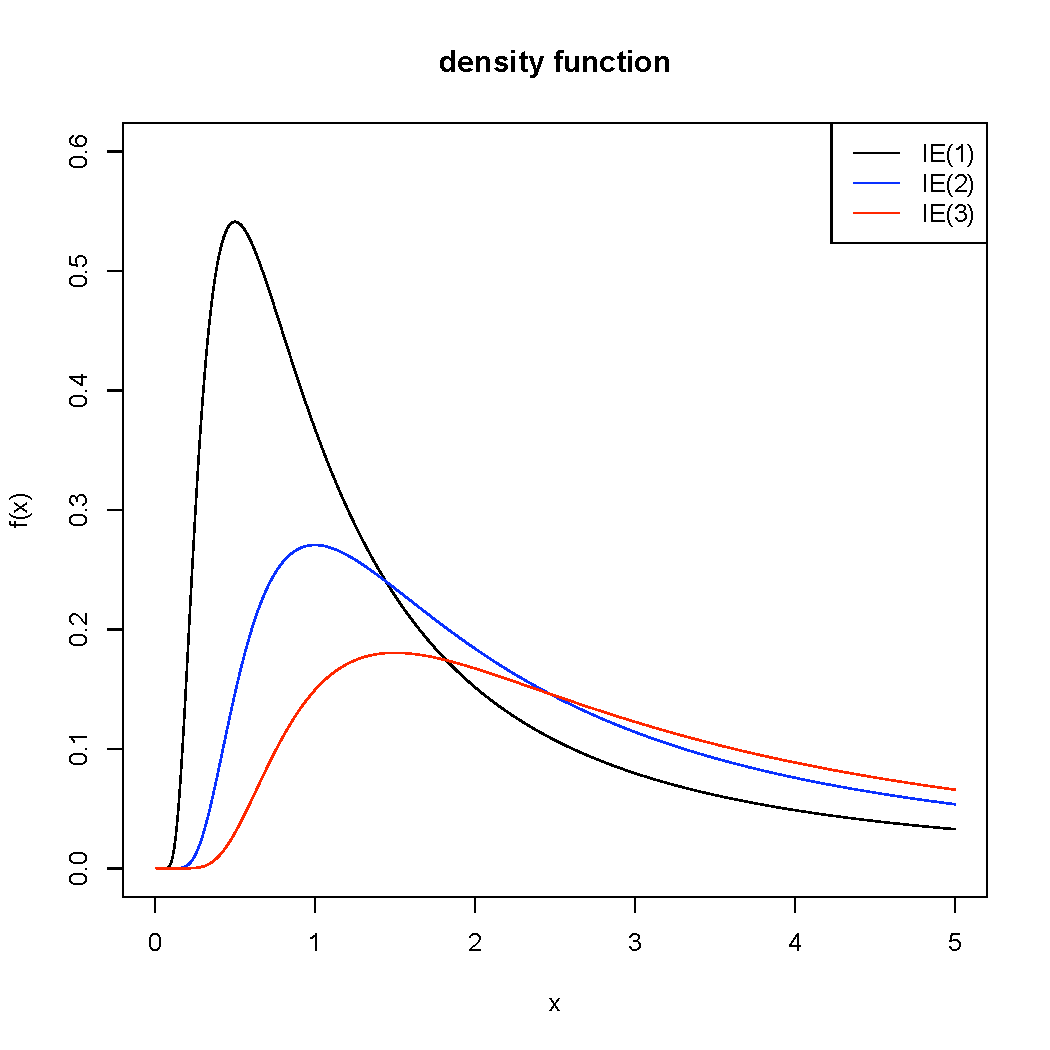
\includegraphics[width=0.48\textwidth]{img/invexpzoom}
  \end{center}
  \vspace{-20pt}  
  \caption{Density function for inverse exponential distributions}
\end{wrapfigure}
This is the distribution of the random variable $\frac{1}{X}$ when $X$ is exponentially distributed. The density defined as
$$
f(x)=\frac{\lambda}{x^2}e^{-\frac{\lambda}{x}},
$$
where $x>0$ and $\lambda>0$. The distribution function can then be derived as 
$$
F(x) =e^{-\frac{\lambda}{x}}.
$$
We can define inverse exponential distributions with characteristic or moment generating functions
$$
\phi(t)=2\sqrt{-it\lambda} K_1\left(2\sqrt{-i \lambda t}\right)
$$
and
$$
M(t)=2\sqrt{-it \lambda} K_1\left(2\sqrt{-\lambda t}\right).
$$
where $K_.(.)$ denotes the modified Bessel function.


\subsection{Properties}
Moments of the inverse exponential distribution are given by
$$
E(X^r) = \lambda^r * \Gamma(1-r)
$$
for $r <1$. Thus the expectation and the variance of the inverse exponential distribution do not exist.

\subsection{Estimation}
Maximum likelihood estimator of $\lambda$ is
$$
\hat \lambda = n \left(\sum_{i=1}^n\frac{1}{X_i} \right)^{-1},
$$
which is also the moment based estimator with $E(X^{-1}) = \lambda^{-1}$.

\subsection{Random generation}
The algorithm is simply to inverse an exponential variate of parameter $\frac{1}{\lambda}$, i.e. $(-\lambda \log(U))^{-1}$ for an uniform variable $U$.

\subsection{Applications}
NEED REFERENCE

%%%%%%%%%%%%%%%%%%%%%%%%%%%%%%%%%%%%%%%%%%%%%%%
\section{Gamma distribution}
\subsection{Characterization}
\begin{wrapfigure}{r}{0.5\textwidth}
  \vspace{-20pt}
  \begin{center}
    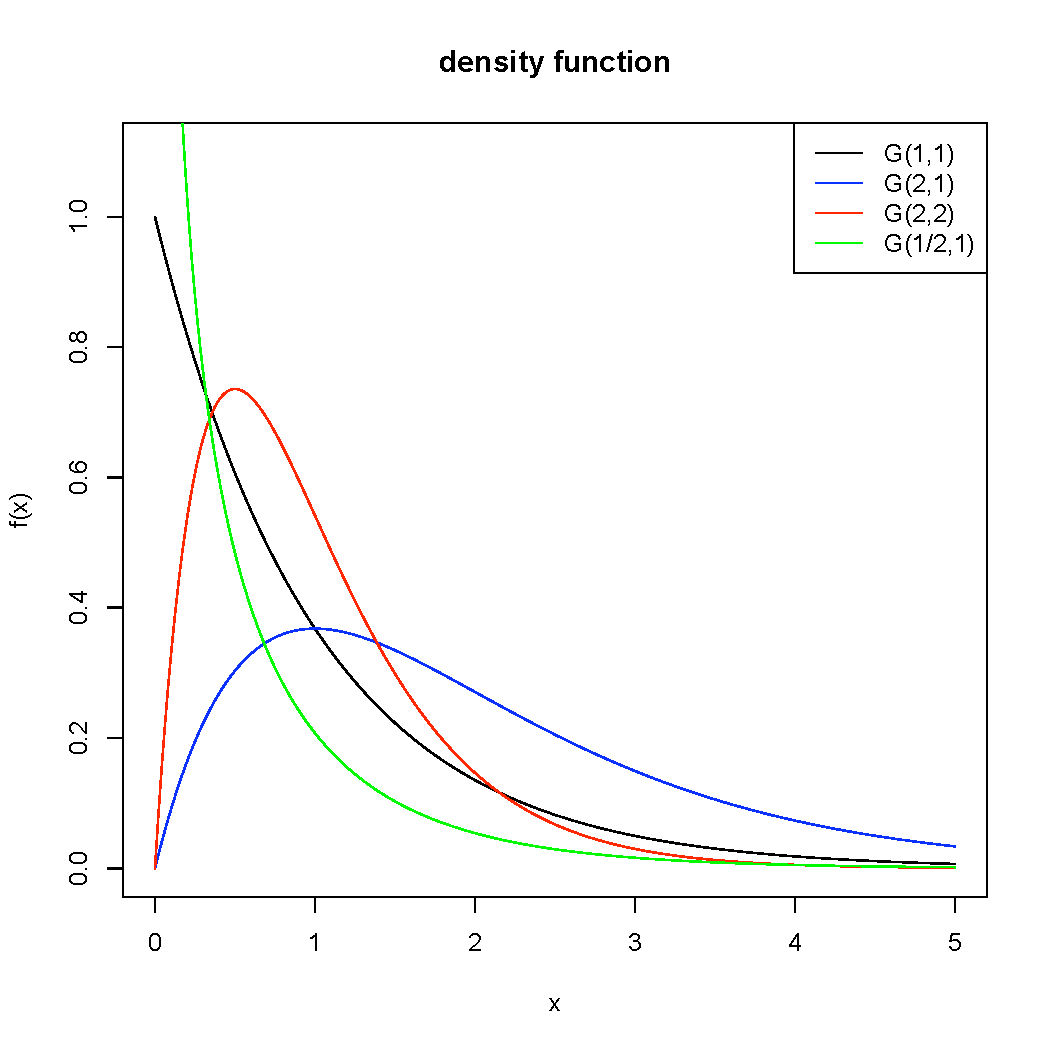
\includegraphics[width=0.48\textwidth]{img/gammazoom}
  \end{center}
  \vspace{-20pt}  
  \caption{Density function for gamma distributions}
\end{wrapfigure}

The gamma distribution is a generalization of the exponential distribution. Its density is defined as
$$
f(x)=\frac{\lambda^{\alpha}}{\Gamma(\alpha)} e^{-\lambda x} x^{\alpha-1},
$$
where $x\geq0$, $\alpha,\lambda>0$ and $\Gamma$ denotes the gamma function. We retrieve the exponential distribution by setting $\alpha$ to 1. When $\alpha$ is an integer, the gamma distribution is sometimes called the Erlang distribution.

The distribution function can be expressed in terms of the incomplete gamma distribution. We get
$$
F(x) = \frac{\gamma(\alpha,\lambda x)}{\Gamma(\alpha)},
$$
where $\gamma(.,.)$ is the incomplete gamma function. 

There is no analytical formula except when we deal with Erlang distribution (i.e. $\alpha \in \mathbb N$). In this case, we have
$$
F(x) = 1-\sum\limits_{i=0}^{\alpha-1} \frac{(\lambda x )^i}{i!}e^{-\lambda x} .
$$

For the gamma distribution, the moment generating and characteristic functions exist.
$$
\phi(t) = \left(\frac{\lambda}{\lambda-it}\right)^{-\alpha},
$$
and
$$
M(t) =\left(\frac{\lambda}{\lambda-t}\right)^{-\alpha}.
$$

\subsection{Properties}
The expectation of a gamma distribution $\mathcal G(\alpha, \lambda)$ is $E(X) = \frac{\alpha}{\lambda}$, while its variance is $Var(X) = \frac{\alpha}{\lambda^2}$. 

For a gamma distribution $\mcal G(\alpha, \lambda)$, the $\tau$th moment is given by
$$
E(X^r) =\lambda^r\frac{\Gamma(\alpha+r)}{\Gamma(\alpha)},
$$
provided that $\alpha+r>0$.

As for the exponential, we have a property on the convolution of gamma distributions. Let $X$ and $Y$ be gamma distributed $\mathcal G(\alpha,\lambda)$ and $\mathcal G(\beta,\lambda)$, we can prove that $X+Y$ follows a gamma distribution $\mathcal G(\alpha+\beta,\lambda)$.

For $X$ and $Y$ gamma distributed ($\mathcal G(\alpha,\lambda)$ and $\mathcal G(\beta,\lambda)$ resp.), we also have that $\frac{X}{X+Y}$ follows a beta distribution of the first kind with parameter $\alpha$ and $\beta$.

\subsection{Estimation}
Method of moments give the following estimators
$$
\tilde \alpha = \frac{(\bar X_n)^2}{S_n^2}
\txtm{and}
\tilde \lambda = \frac{\bar X_n}{S_n^2}.
$$
with $\bar X_n$ and $S_n^2$ the sample mean and variance.

Maximum likelihood estimators of $\alpha,\lambda$ verify the system
$$
\left\{
\begin{array}{l}
\log \alpha- \psi(\alpha)=    \log(\frac{1}{n}\sum_{i=1}^n X_i) -\frac{1}{n}\sum_{i=1}^n \log X_i \\
\lambda =\frac{n\alpha}{\sum_{i=1}^n X_i}\\
\end{array}
\right. ,
$$
where $\psi(.)$ denotes the digamma function. The first equation can be solved numerically\footnote{algorithm can be initialized with $\tilde \alpha$.} to get $\hat \alpha$ and then $\hat \lambda = \frac{\hat \alpha}{\bar X_n}$. But $\hat \lambda$ is biased, so the unbiased estimator with minimum variance of $\lambda$ is 
$$
\bar \lambda = \frac{\hat \alpha n}{\hat \alpha n -1}\frac{\hat \alpha}{\bar X_n}
$$

NEED REFERENCE for confidence interval

\subsection{Random generation}
Simulate a gamma $\mcal G(\alpha, \lambda)$ is quite tricky for non integer shape parameter. Indeed, if the shape parameter $\alpha$ is integer, then we simply sum $\alpha$ exponential random variables $\mcal E(\lambda)$. Otherwise we need to add a gamma variable $\mcal G(\alpha -\lfloor \alpha \rfloor, \lambda)$.
This is carried out by an acceptance/rejection method.

NEED REFERENCE

\subsection{Applications}
NEED REFERENCE

%%%%%%%%%%%%%%%%%%%%%%%%%%%%%%%%%%%%%%%%%%%%%
\section{Generalized Erlang distribution}

\subsection{Characterization}
\begin{wrapfigure}{r}{0.5\textwidth}
  \vspace{-30pt}
  \begin{center}
    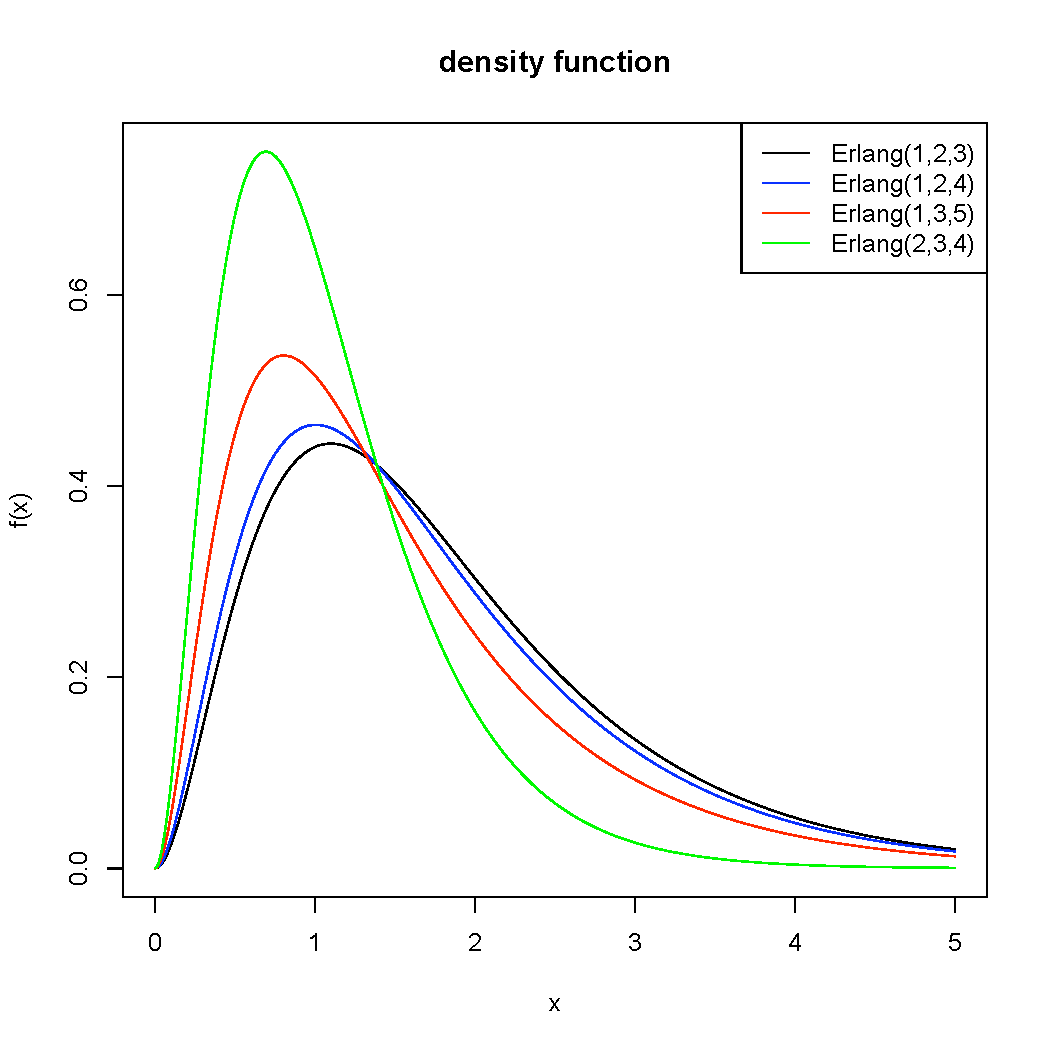
\includegraphics[width=0.48\textwidth]{img/generlangzoom}
  \end{center}
  \vspace{-20pt}  
  \caption{Density function for generalized Erlang distributions}
    \vspace{-20pt}  
\end{wrapfigure}

As the gamma distribution is the distribution of the sum of i.i.d. exponential distributions, the generalized Erlang distribution is the distribution of the sum independent exponential distributions. Sometimes it is called the hypoexponential distribution. The density is defined as 
$$
f(x) = \sum\limits_{i=1}^{d} \left( \prod\limits_{j=1,j\neq i}^d \frac{\lambda_j }{\lambda_j -\lambda_i} \right)\lambda_i e^{-\lambda_i x},
$$
where $x\geq 0$ and $\lambda_j>0$'s\footnote{with the constraint that all $\lambda_j$'s are strictly different.} are the paremeters (for each exponential distribution building the generalized Erlang distribution). There is an explicit form for the distribution function:
$$
F(x) = \sum\limits_{i=1}^{d} \left( \prod\limits_{j=1,j\neq i}^d \frac{\lambda_j }{\lambda_j -\lambda_i} \right)(1-e^{-\lambda_i x}).
$$
This distribution is noted $\mcal Erlang(\lambda_1,\dots, \lambda_d)$. Of course, we retrieve the Erlang distribution when $\forall i, \lambda_i=\lambda$.

Finally, the characteristic and moment generating functions of generalized Erlang distribution are
$$
\phi(t) = \prod\limits_{j=1}^d \frac{\lambda_j  }{\lambda_j -i t} \txtm{and} M(t)=\prod\limits_{j=1}^d \frac{\lambda_j  }{\lambda_j -t}.
$$

\subsection{Properties}
The expectation of the generalized Erlang distribution is simply $E(X) =\sum\limits_{i=1}^d\frac{1}{\lambda_i}$ and its variance $Var(X) = \sum\limits_{i=1}^d\frac{1}{\lambda_i^2}$.
 
 
\subsection{Estimation}
NEED REFERENCE

\subsection{Random generation}
The algorithm is very easy simulate independently $d$ random variables exponentially $\mcal E(\lambda_j)$ distributed and sum them.

\subsection{Applications}
NEED REFERENCE

%%%%%%%%%%%%%%%%%%%%%%%%%%%%%%%%%%%%%%%%%%%%%%
\section{Chi-squared distribution}
A special case of the gamma distribution is the chi-squared distribution. See section \ref{chisquared}.


%%%%%%%%%%%%%%%%%%%%%%%%%%%%%%%%%%%%%%%%%%%%%%
\newpage
\section{Inverse Gamma}
\subsection{Characterization}
\begin{wrapfigure}{r}{0.5\textwidth}
  \vspace{-20pt}
  \begin{center}
    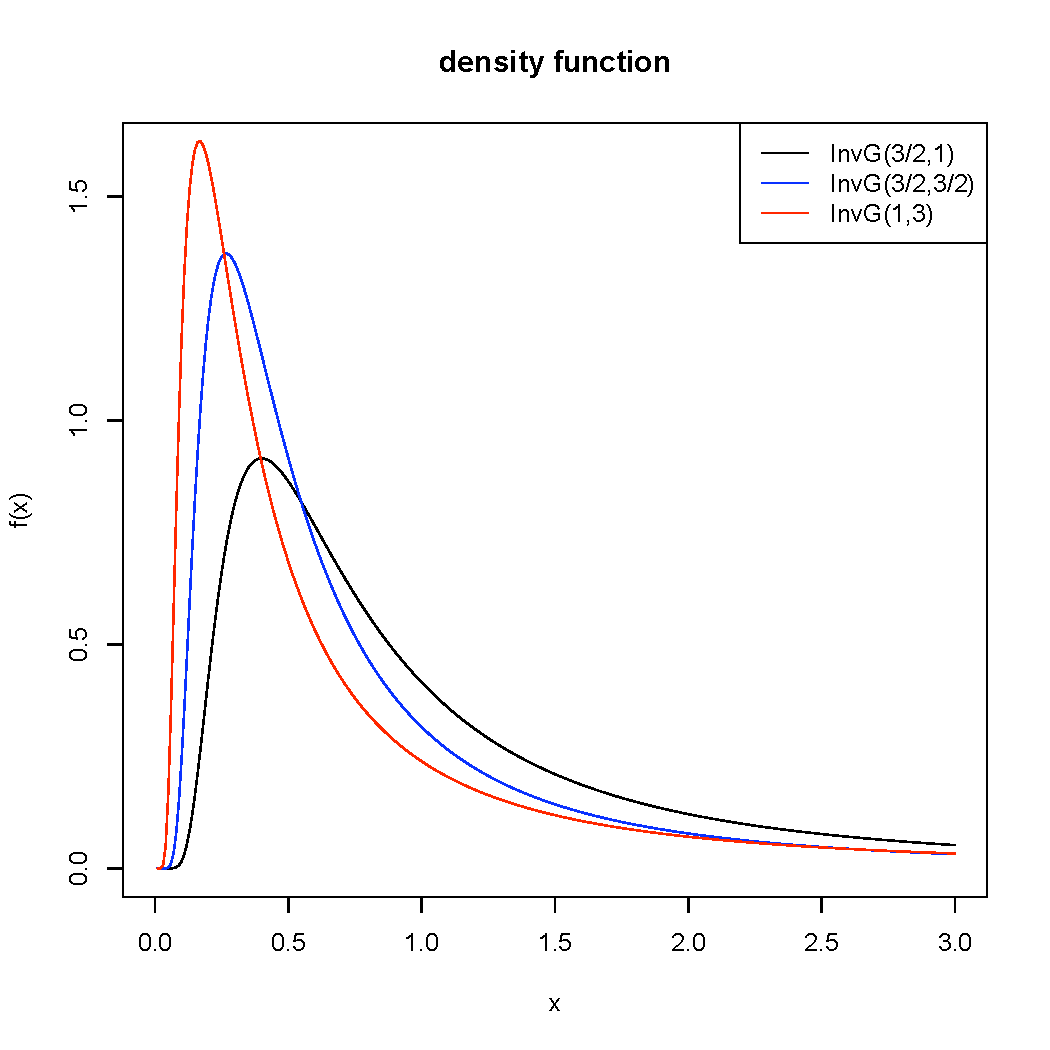
\includegraphics[width=0.48\textwidth]{img/invgammazoom}
  \end{center}
  \vspace{-20pt}  
  \caption{Density function for inverse gamma distributions}  
\end{wrapfigure}

The inverse gamma distribution is the distribution of a random variable $\frac{1}{X}$ when $X$ is gamma distributed. Hence the density is 
$$
f(x)=\frac{\lambda^\alpha}{\Gamma(\alpha)x^{\alpha+1}}e^{-\frac{\lambda}{x}},
$$
where $x>0$ and $\beta,\alpha>0$. From this, we can derive the distribution function 
$$
F(x)=\frac{\gamma(\alpha,\frac{\lambda}{x})}{\Gamma(\alpha)}.
$$

We can define inverse gamma distributions with characteristic or moment generating functions
$$
\phi(t)=\frac{2\sqrt{-it \lambda}^{\alpha}}{\Gamma(\alpha)} K_\alpha(2\sqrt{-i \lambda t})
$$
and
$$
M(t)=\frac{2\sqrt{-it \lambda}^{\alpha}}{\Gamma(\alpha)} K_\alpha(2\sqrt{-\lambda t}).
$$
where $K_.(.)$ denotes the modified Bessel function.

\subsection{Properties}
The expectation exists only when $\alpha>1$ and in this case $E(X)=\frac{\lambda}{\alpha-1}$, whereas the variance is only finite if $\alpha >2$ and $Var(X) = \frac{\lambda ^2}{(\alpha-1)^2(\alpha-2)}$.

\subsection{Estimation}
Method of moments give the following estimators
$$
\tilde \alpha = 2+\frac{(\bar X_n)^2}{S_n^2}
\txtm{and}
\tilde \lambda = \bar X_n(\tilde \alpha -1)
$$
with $\bar X_n$ and $S_n^2$ the sample mean and variance. If the variance does not exist, then $\alpha$ will be 2, it means we must use the maximum likelihood estimator (which works also for $\alpha\leq 2$).

Maximum likelihood estimators of $\alpha,\lambda$ verify the system
$$
\left\{
\begin{array}{l}
\log \alpha- \psi(\alpha)=    \log(\frac{1}{n}\sum_{i=1}^n \frac{1}{X_i}) -\frac{1}{n}\sum_{i=1}^n \log \frac{1}{X_i} \\
\lambda =\alpha \left(\frac{1}{n}\sum_{i=1}^n \frac{1}{X_i}\right)^{-1}
\end{array}
\right. ,
$$
where $\psi(.)$ denotes the digamma function. The first equation can be solved numerically\footnote{algorithm can be initialized with $\tilde \alpha$.} to get $\hat \alpha$ and then $\hat \lambda$ with the second equation.



\subsection{Random generation}
Simply generate a gamma variable $\mcal G(\alpha, 1/\lambda)$ and inverse it.

\subsection{Applications}
NEED REFERENCE



%%%%%%%%%%%%%%%%%%%%%%%%%%%%%%%%%%%%%%%%%%%%%%%%
\section{Transformed or generalized gamma}
\subsection{Characterization}
\begin{wrapfigure}{r}{0.5\textwidth}
  \vspace{-20pt}
  \begin{center}
    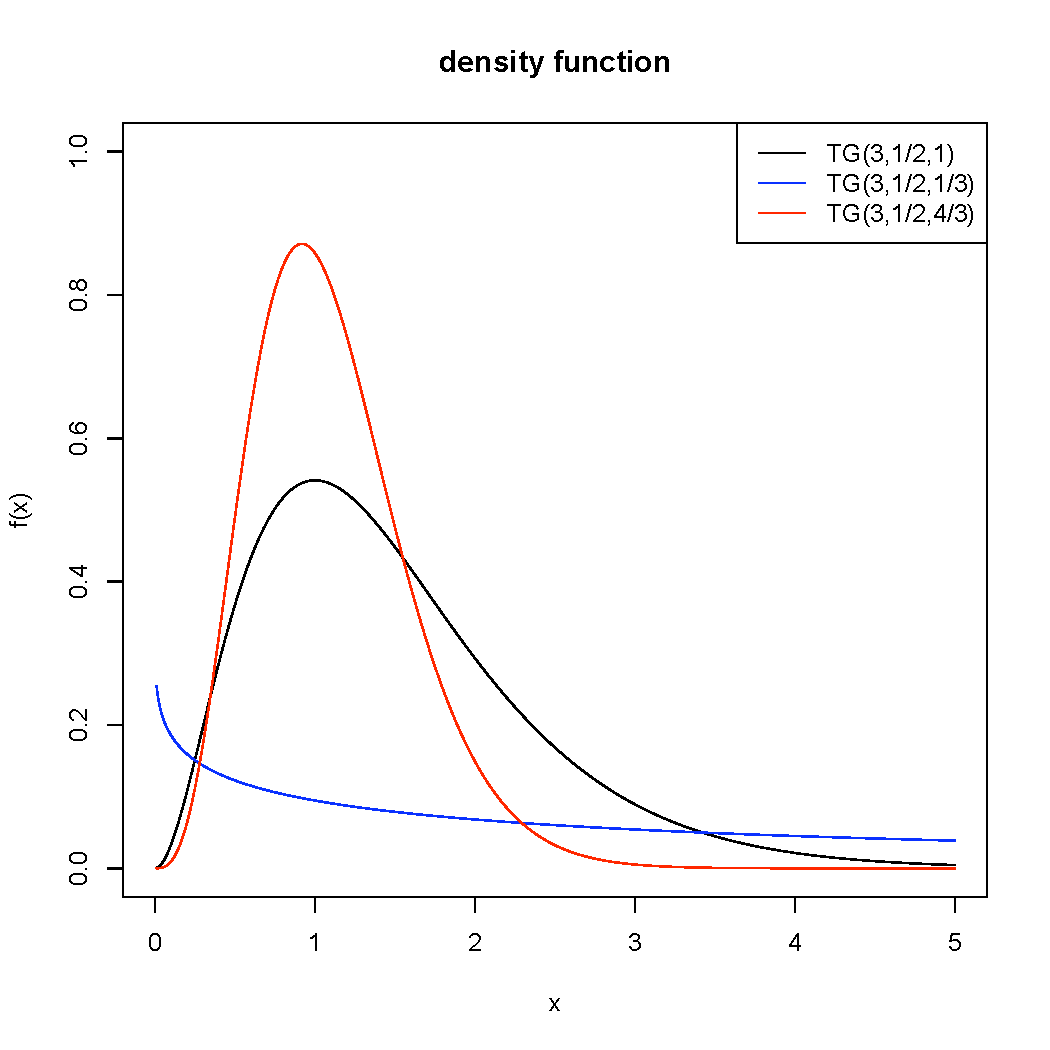
\includegraphics[width=0.48\textwidth]{img/transgammazoom}
  \end{center}
  \vspace{-20pt}  
  \caption{Density function for transformed gamma distributions}  
\end{wrapfigure}

The transformed gamma distribution is defined by the following density function
$$
f(x)=\frac{\tau (\frac{x}{\lambda})^{\alpha\tau-1} e^{-(\frac{x}{\lambda})^{\tau}} }{\lambda\Gamma(\alpha)},
$$
where $x>0$ and $\alpha, \lambda, \tau >0$. Thus, the distribution function is 
$$
F(x) = \frac{\gamma(\alpha,(\frac{x}{\lambda})^{\tau})}{\Gamma(\alpha)}.
$$
This is the distribution of the variable $\lambda X^{\frac{1}{\tau}}$ when $X$ is gamma distributed $\mcal G(\alpha,1)$.

Obviously, a special case of the transformed gamma is the gamma distribution with $\tau=1$. But we get the Weibull distribution with $\alpha=1$.

\subsection{Properties}
The expectation of the transformed gamma distribution is $E(X)=\frac{\lambda\Gamma(\alpha+\frac{1}{\tau})}{\Gamma(\alpha)}$ and its variance $Var(X)=\frac{\lambda^2\Gamma(\alpha+\frac{2}{\tau})}{\Gamma(\alpha)}-E^2[X]$.

From \cite{venter} moments are given by
$$
E(X^r) = \lambda^r \frac{\Gamma(\alpha+\frac{r}{\tau})}{\Gamma(\alpha)},
$$
with $\alpha+\frac{r}{\tau}>0$.

\subsection{Estimation}
Maximum likelihood estimators verify the following system
$$
\left\{
\begin{array}{l}
\psi(\alpha) - \log \alpha = \tau \frac{1}{n} \sum\limits_{i=1}^n \log X_i- \log(\frac{1}{n} \sum\limits_{i=1}^n X_i^\tau ) \\
\alpha = \frac{1}{n} \sum\limits_{i=1}^n X_i^\tau \left(  \frac{1}{n} \sum\limits_{i=1}^n X_i^\tau \log X_i -\left(\frac{1}{n} \sum\limits_{i=1}^n X_i^\tau \right) \left( \frac{1}{n} \sum\limits_{i=1}^n \log X_i\right) \right)^{-1} \\
\lambda = \left(\frac{1}{n} \sum\limits_{i=1}^n X_i^\tau \right)^\tau \alpha^{-\tau}
\end{array}
\right. ,
$$
where $\psi$ denotes the digamma function. This system can be solved numerically. 

TODO : use \cite{dussauchoy}

\subsection{Random generation}
Generate a gamma distributed variable ($\mcal G(\alpha,1)$),  raise it to power $\frac{1}{\tau}$ and multiply it by $\lambda$.

\subsection{Applications}
In an actuarial context, the transformed gamma may be useful in loss severity, for example, in workers' compensation, see \cite{venter}.

%%%%%%%%%%%%%%%%%%%%%%%%%%%%%%%%%%%%%%%%%%
\newpage
\section{Inverse transformed Gamma}
\subsection{Characterization}
\begin{wrapfigure}{r}{0.5\textwidth}
  \vspace{-20pt}
  \begin{center}
    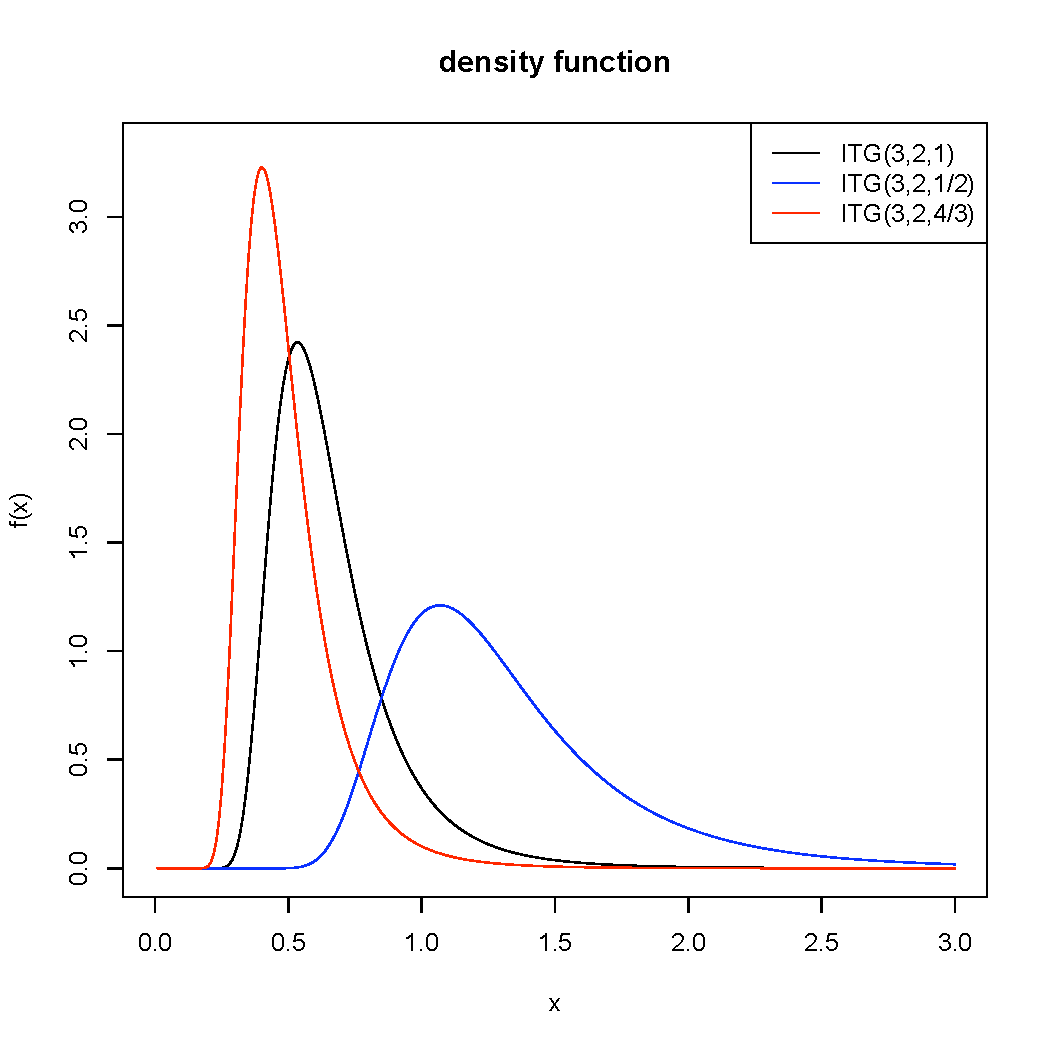
\includegraphics[width=0.48\textwidth]{img/invtrgammazoom}
  \end{center}
  \vspace{-20pt}  
  \caption{Density function for inverse transformed gamma distributions}  
\end{wrapfigure}
The transformed gamma distribution is defined by the following density function
$$
f(x)=\frac{\tau (\frac{\lambda}{x})^{\alpha\tau} e^{-(\frac{\lambda}{x})^{\tau}} }{x\Gamma(\alpha)},
$$
where $x>0$ and $\alpha, \lambda, \tau >0$. Thus, the distribution function is 
$$
F(x) = 1-\frac{\gamma(\alpha,(\frac{\lambda}{x})^{\tau})}{\Gamma(\alpha)}.
$$
This is the distribution of $\left(\frac{\lambda}{X}\right)^\frac{1}{\tau}$ when $X$ is gamma distributed $\mcal G(\alpha,1)$.
\subsection{Properties}
The expectation of the transformed gamma distribution is $E(X)=\frac{\lambda\Gamma(\alpha-\frac{1}{\tau})}{\Gamma(\alpha)}$ and its variance $Var(X)=\frac{\lambda^2\Gamma(\alpha-\frac{2}{\tau})}{\Gamma(\alpha)}-E^2[X]$.

From \cite{klugman}, we have the following formula for the moments
$$
E(X^r) = \frac{\lambda^r\Gamma(\alpha-\frac{r}{\tau})}{\Gamma(\alpha)}.
$$


\subsection{Estimation}
NEED REFERENCE
\subsection{Random generation}
Simply simulate a gamma $\mcal G(\alpha,1)$ distributed variable, inverse it, raise it to power $\frac{1}{\alpha}$ and multiply it by $\lambda$.

\subsection{Applications}
NEED REFERENCE

%%%%%%%%%%%%%%%%%%%%%%%%%%%%%%%%%%%%%%%%%%
\section{Log Gamma}
\subsection{Characterization}
Density function for log-gamma distribution is expressed as
$$
f(x) = \frac{e^{k\frac{x-a}{b} -e^{\frac{x-a}{b}} }}{\Gamma(k)}
$$
for $x>0$, where $a$ is the location parameter, $b>0$ the scale parameter and $k>0$ the shape parameter. The distribution function is 
$$
F(x) = \frac{\gamma(k, e^{\frac{x-a}{b}})}{\Gamma(k)},
$$
for $x>0$. This is the distribution of $a+b\log(X)$ when $X$ is gamma $\mcal G(k,1)$.

\subsection{Properties}
The expectation is $E(X)=a+b\psi(k)$ and the variance $Var(X) =b^2\psi_1(k)$ where $\psi$ is the digamma function and $\psi_1$ the trigamma function.

\subsection{Estimation}
NEED REFERENCE

\subsection{Random generation}
Simply simulate a gamma $\mcal G(k,1)$ distributed variable and returns $a+b\log(X)$.

\subsection{Applications}
NEED REFERENCE


%%%%%%%%%%%%%%%%%%%%%%%%%%%%%%%%%%%%%%%%%%%
\section{Weibull distribution}\label{weibull}
\subsection{Characterization}
\begin{wrapfigure}{r}{0.5\textwidth}
  \vspace{-40pt}
  \begin{center}
    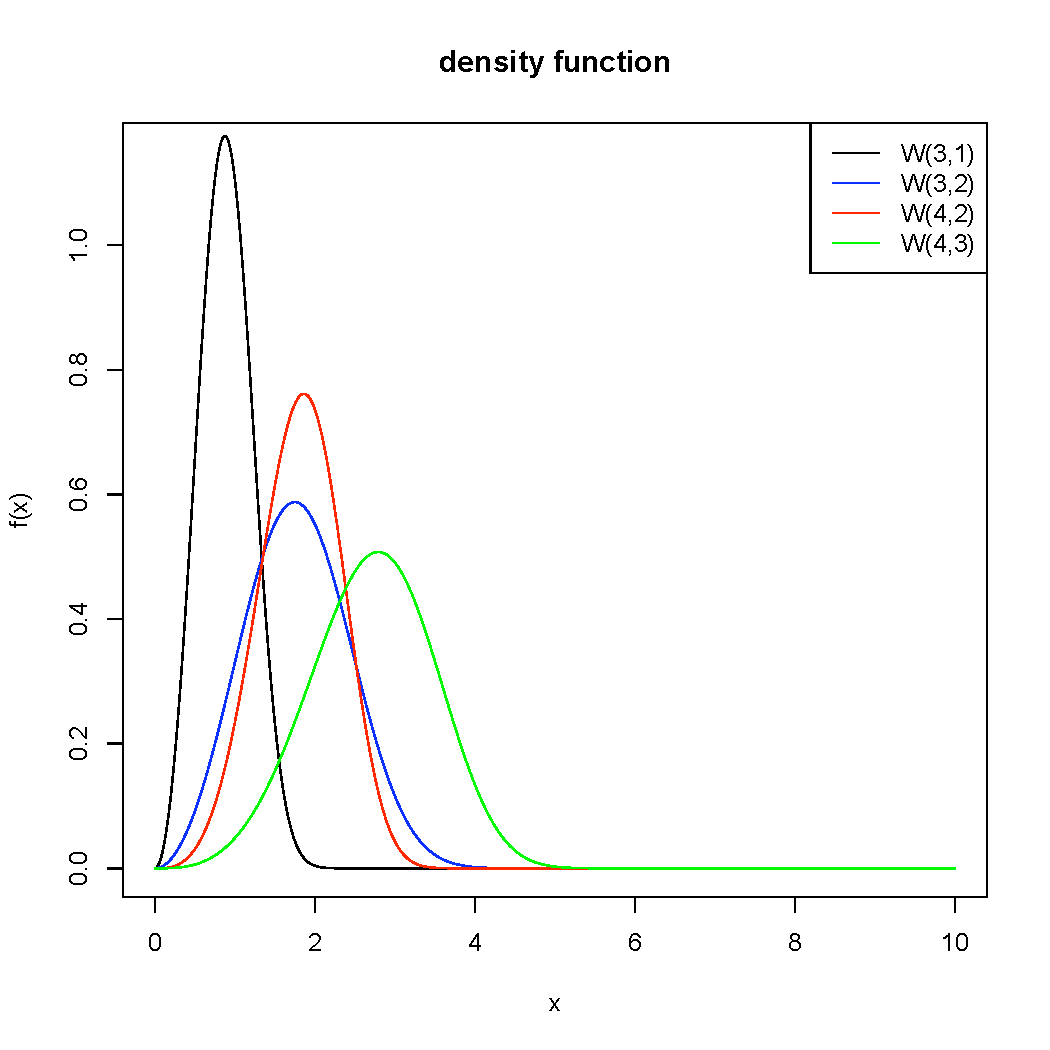
\includegraphics[width=0.48\textwidth]{img/weibullzoom}
  \end{center}
  \vspace{-20pt}  
  \caption{Density function for Weibull distributions}  
\end{wrapfigure}

Despite the fact the Weibull distribution is not particularly related to the chi distribution, its density tends exponentially fast to zero, as chi's related distribution. The density of a Weibull distribution is given by
$$
f(x) = \frac{\beta  }{\eta^{\beta}} x^{\beta-1} e^{-(\frac{x}{\eta})^{\beta}},
$$
where $x>0$ and $\eta, \beta >0$.
In terms of distribution function, the Weibull can be defined as
$$
F(x) =1-e^{-(\frac{x}{\beta})^\eta}.
$$

There exists a second parametrization of the Weibull distribution. We have
$$
f(x) = \tau \lambda x^{\lambda-1} e^{-\tau x^{\lambda}},
$$
with the same constraint on the parameters $\tau, \lambda >0$. In this context, the distribution function is 
$$
F(x) = 1-e^{-\tau x^{\lambda}}.
$$
We can pass from the first parametrization to the second one with
$$
\left\{
\begin{array}{c}
\lambda = \beta\\
\tau = \frac{1}{\eta^\beta}
\end{array}
\right. .
$$

\subsection{Properties}
The expectation of a Weibull distribution $\mathcal{ W}(\eta,\beta)$ is $E(X) = \eta \Gamma(1+\frac{1}{\beta})$ and the variance $Var(X) = \eta^2[\Gamma(\frac{\beta+2}{\beta})-\Gamma(\frac{\beta+1}{\beta})^2]$. In the second parametrization, we have $E(X) =  \frac{\tau(1+\frac{1}{\tau})}{\lambda^{\frac{1}{\tau}}}$ and $Var(X) = \frac{1}{\lambda^{\frac{2}{\tau}}}(\tau(1+\frac{2}{\tau}) - \tau(1+\frac{1}{\tau})^2)$.

The $r$th raw moment $E(X^r)$ of the Weibull distribution $\mathcal{ W}(\eta,\beta)$ is given by $\eta \Gamma(1+\frac{r}{\beta})$ for $r>0$.

The Weibull distribution is the distribution of the variable $\frac{X^\beta}{\eta}$ where $X$ follows an exponential distribution $\mathcal E(1)$.

\subsection{Estimation}
We work in this sub-section with the first parametrization. From the cumulative distribution, we have
$$
\log(-\log|1-F(x)|) = \beta\log x-\beta \log \eta.
$$
Thus we can an estimation of $\beta$ and $\eta$ by regressing $ \log(-\log{|\frac{i}{n}|})$ on $\log X_{i:n}$.
Then we get the following estimators
$$
\tilde \beta = \hat a \txtm{and} \tilde \eta = e^{-\frac{\hat b}{\hat a}},
$$
where $\hat a$ and $\hat b$ are respectively the slope and the intercept of the regression line.

The maximum likelihood estimators verify the following system
$$
\left\{
\begin{array}{l}
- \frac{n\beta}{\eta}+\frac{\beta}{\eta^{\beta+1}} \sum_{i=1}^{n}(x_i)^{\beta} = 0\\
 \frac{n}{\beta} -n\ln(\eta)+\sum_{i=1}^{n}\ln(x_i)-\sum_{i=1}^{n}\ln(x_i)(\frac{x_i}{\eta})^{\beta} = 0\\
\end{array}
\right. ,
$$
which can be solved numerically (with algorithm initialized by the previous estimators).

\subsection{Random generation}
Using the inversion function method, we simply need to compute $\beta(-\log(1-U))^{\frac{1}{\eta}}$ for the first parametrization or $\left(\frac{-\log(1-U)}{\tau}\right)^{\frac{1}{\lambda}}$ for the second one where $U$ is an uniform variate.

\subsection{Applications}
The Weibull was created by Weibull when he studied machine reliability.

NEED REFERENCE

%%%%%%%%%%%%%%%%%%%%%%%%%%%%%%%%%%%%%%%%%%%
\section{Inverse Weibull distribution}\label{invweibull}
\subsection{Characterization}
\begin{wrapfigure}{r}{0.5\textwidth}
  \vspace{-40pt}
  \begin{center}
    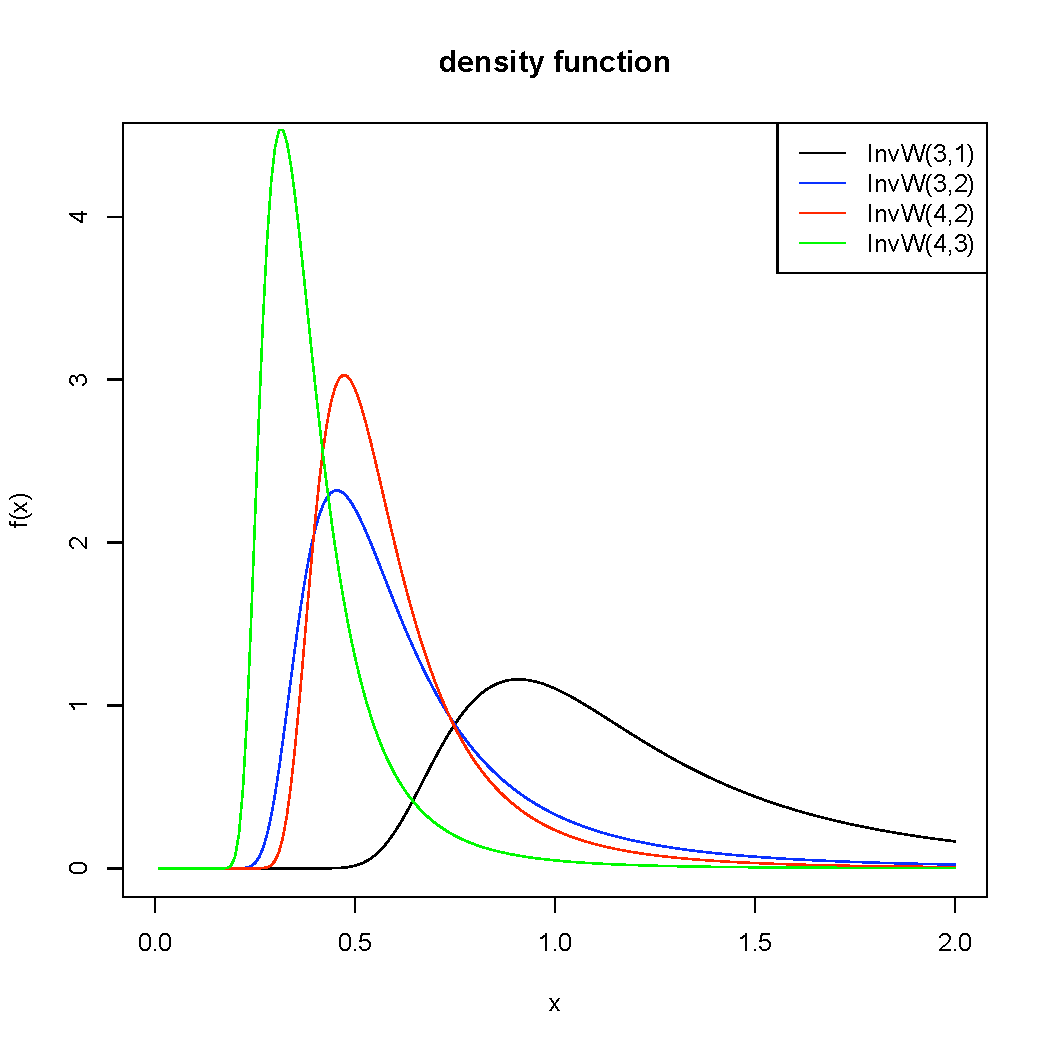
\includegraphics[width=0.48\textwidth]{img/invweibullzoom}
  \end{center}
  \vspace{-20pt}  
  \caption{Density function for inverse Weibull distributions}  
\end{wrapfigure}

The inverse Weibull distribution is defined as
$$
f(x) = \frac{\eta \beta^\eta e^{-(\frac{\beta}{x})^\eta} }{x^{\eta+1}},
$$
where $x>0$ and $\eta, \beta >0$. Its distribution function is
$$
F(x) = e^{-(\frac{\beta}{x})^\eta}.
$$
This is the distribution of $1/X$ when $X$ is Weibull distributed $\mcal W(\beta^{-1},\eta)$.

\subsection{Properties}
The expectation is given by $\eta \Gamma(1-\frac{1}{\beta})$ and the variance $\eta^2[\Gamma(\frac{\beta-2}{\beta})-\Gamma(\frac{\beta-1}{\beta})^2]$.

The $r$th moment of the Weibull distribution $\mathcal I\mathcal{W}(\eta,\beta)$ is given by $\eta^r \Gamma(1-\frac{r}{\beta})$ for $r>0$.

\subsection{Estimation}
Maximum likelihood estimators for $\beta$ and $\eta$ verify the following system
$$
\left\{
\begin{array}{l}
\frac{1}{\beta} = \frac{1}{n} \sum_{i=1}^n�\left( \frac{\beta}{X_i} \right)^{\eta-1} \\
\frac{1}{\eta} + \log(\beta) = \frac{1}{n} \sum_{i=1}^n \left( \frac{\beta}{X_i} \right)^{\eta} \log\left( \frac{\beta}{X_i} \right) + \frac{1}{n}\sum_{i=1}^n \log(X_i)
\end{array}
\right. ,
$$
while the method of moment has the following system
$$
\left\{
\begin{array}{l}
(S_n^2+(\bar X_n)^2) \Gamma^2(1-\frac{1}{\beta}) = (\bar X_n)^2 \Gamma(1-\frac{2}{\beta}) \\
\eta = \frac{\bar X_n}{\Gamma(1-\frac{1}{\beta})}
\end{array}
\right. .
$$
Both are to solve numerically.

\subsection{Random generation}
Simply generate a Weibull variable $\mcal W(\beta^{-1},\eta)$ and inverse it.

\subsection{Applications}
NEED REFERENCE

TODO \cite{ortega}

%%%%%%%%%%%%%%%%%%%%%%%%%%%%%%%%%%%%%%%%%%
\section{Laplace or double exponential distribution}
\subsection{Characterization}
\begin{wrapfigure}{r}{0.5\textwidth}
  \vspace{-20pt}
  \begin{center}
    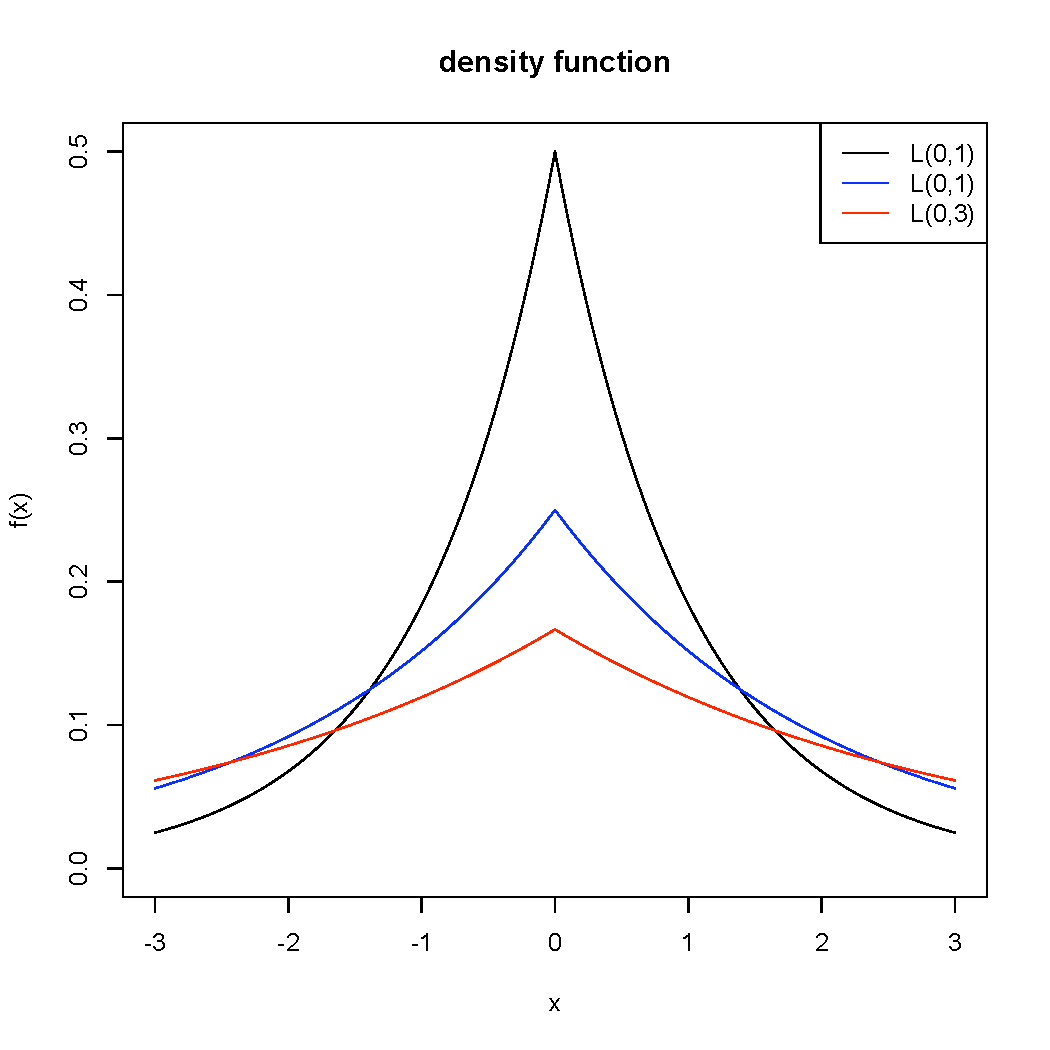
\includegraphics[width=0.48\textwidth]{img/laplacezoom}
  \end{center}
  \vspace{-20pt}  
  \caption{Density function for laplace distributions}  
\end{wrapfigure}

Density for the Laplace distribution is given by
$$
f(x) = \frac{1}{2\sigma^2} e^{-\frac{|x-m|}{\sigma} }, 
$$
for $x\in\mbb R$, $m$ the location parameter and $\sigma>0$ the scale parameter.
We have the following distribution function 
$$
F(x) = \left\{
\begin{array}{ll}
\frac{1}{2}e^{-\frac{m-x}{\sigma}} &\txtm{if} x<m\\
1-\frac{1}{2}e^{-\frac{x-m}{\sigma}} & \txtm{otherwise}\\
\end{array}
\right. .
$$
There exists a moment generating function for this distribution, which is
$$
M(t) = \frac{e^{mt}}{1-\sigma^2t^2},
$$
for $|t|< \frac{1}{\sigma}$.
The characteristic function is expressed as 
$$
\phi(t) = \frac{e^{imt}}{1+\sigma^2t^2},
$$
for $t\in\mbb R$.


\subsection{Properties}
The expectation for the Laplace distribution is given by $E(X) = m$ while the variance is $Var(X)=2\sigma^2$.

\subsection{Estimation}
Maximum likelihood estimators for $m$ and  $\sigma$ are 
$$
\hat m =\left\{
\begin{array}{ll}
\frac{X_{\frac{n}{2}:n}+X_{\frac{n+2}{2}:n}}{2} &\txtm{if} n \txtm{is even}\\
X_{\lfloor \frac{n}{2}\rfloor :n} & \txtm{otherwise}\\
\end{array}
\right. ,
$$
where $X_{k:n}$ denotes the $k$th order statistics and 
$$
\hat \sigma = \frac{1}{n} \sum_{i=1}^n|X_i -\hat m|.
$$

\subsection{Random generation}
Let $U$ be a uniform variate. Then the algorithm is
\begin{itemize}
\item $V = U-1/2$
\item $X=m+\sigma \textrm{sign}(V)\log(1-2|V|)$
\item return $X$
\end{itemize}


\subsection{Applications}
NEED 

 The Double Exponential Distribution: Using Calculus to Find a Maximum Likelihood Estimator
 Robert M. Norton
 The American Statistician, Vol. 38, No. 2 (May, 1984), pp. 135-136 

